\newpage
\chapter{Notions}
\label{chap:notions}

Le domaine d'activité entourant ce stage est très riche en matière de notion et de vocabulaire. Ainsi, afin de mieux comprendre de quoi il va être question tout au long de ce rapport, il est nécessaire d'en définir les notions de base.

\paragraph{Réalité virtuelle}
La réalité virtuelle\cite{milgram1995augmented}, plus communément appelée \emph{Virtual Reality (VR)}, désigne l'ensemble des environnements purement numérique (fig~\ref{fig:realityspectrum}, qu'ils soient réalistes ou non, dans lesquels aucune interaction avec l'environnement réel n'est possible et inversement. Cette réalité se base très généralement sur l'utilisation d'un casque \emph{Head Mounted Display (HMD)} dont l'utilisateur doit se munir afin d'être immergé dans un monde numérique avec lequel il peut interagir. L'immersion est le but de la réalité virtuelle.

\begin{figure}[H]
\centering
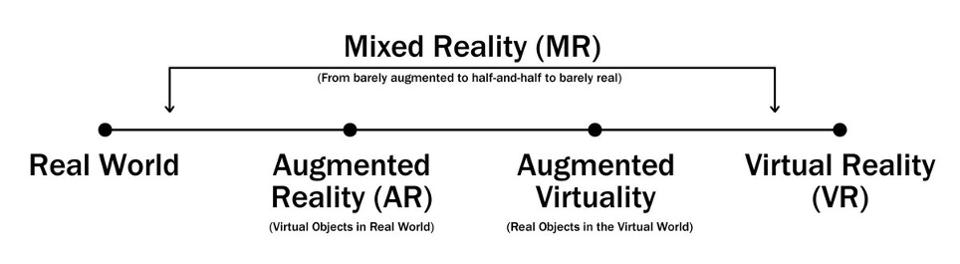
\includegraphics[width=\linewidth]{images/RealitySpectrum}
\caption{Représentation de continuum de la virtualité par Milgram et Kishino, 1995\cite{milgram1995augmented}}
\label{fig:realityspectrum}
\end{figure}

\paragraph{Réalité augmentée}
La réalité augmentée\cite{milgram1995augmented}, plus communément appelée \emph{Augmented Reality (AR)}, quant à elle, est un sous-domaine de la réalité virtuelle. L'idée de la réalité augmentée est de superposer à l'environnement réel des éléments virtuels qui vont alors venir "augmenter" notre monde, en apportant le plus souvent des compléments d'information. Elle est donc qualifiée de sous-domaine de la réalité virtuelle car l'utilisateur n'est plus immergé dans un environnement complètement numérique, mais du contenu virtuel est ajouté en contexte à la vision réelle. Par abus de langage, le terme de réalité augmentée est souvent utilisé pour parler de réalité mixte dont la notion est détaillée dans cette partie.
Il faut noter que ce type de réalité ne se base pas uniquement sur des \emph{HMD} mais peut également être appréciée à l'aide d'un téléphone par exemple (fig~\ref{fig:AR}).

\begin{figure}[H]
\centering
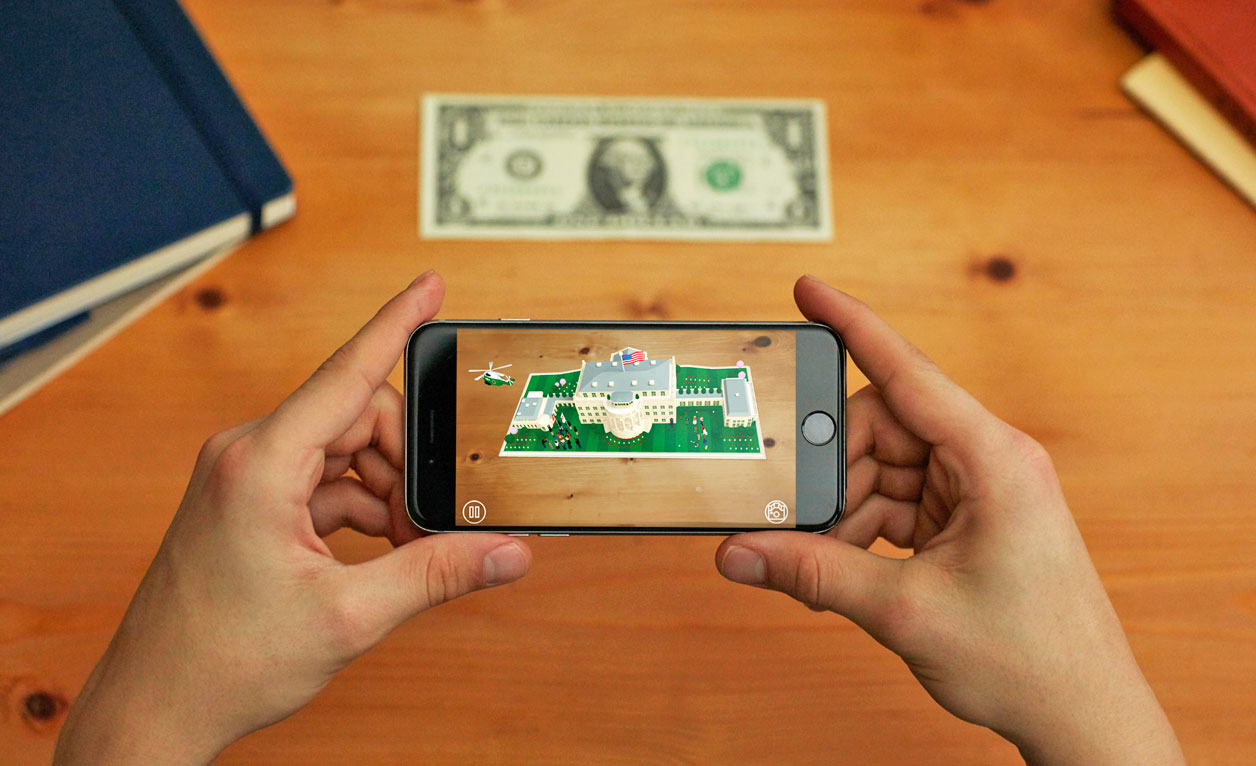
\includegraphics[width=0.55\textwidth]{images/AR}
\caption{Réalité augmentée vue au travers d'un téléphone\protect\footnotemark}\label{fig:AR}
\end{figure}
\footnotetext{Source: \href{https://www.engadget.com}{https://www.engadget.com}}

\paragraph{Réalité mixte}
La réalité mixte, ou hybride, plus communément appelée \emph{Mixed Reality (MR)}, ou \emph{Crossed Reality (XR)}, est la fusion parfaite de l'environnement numérique et de l'environnement physique (fig~\ref{fig:realityspectrum}). Dans ce "nouvel" environnement, les objets physiques et numériques coexistent et peuvent interagir entre eux (par exemple, une table peut devenir une plateforme pour un personnage virtuel (fig~\ref{fig:youngconker})). Souvent confondue avec la réalité augmentée, la différence se situe principalement dans le fait que la réalité mixte ne propose pas seulement une visualisation des objets numériques, elle propose aussi des méthodes d'interaction avec ce contenu. C'est donc la notion d'interaction avec les éléments virtuels qui permet de les différencier. 

A l'heure actuelle, la réalité mixte nécessite un dispositif de type \emph{HMD} pour être appréciée. C'est le cas notamment de l'\texttt{HoloLens} de \texttt{Microsoft}, un casque permettant la superposition d'éléments virtuels au champ de vision de l'utilisateur et permettant également l'interaction entre le monde virtuel et la réalité.

\begin{figure}[H]
\centering
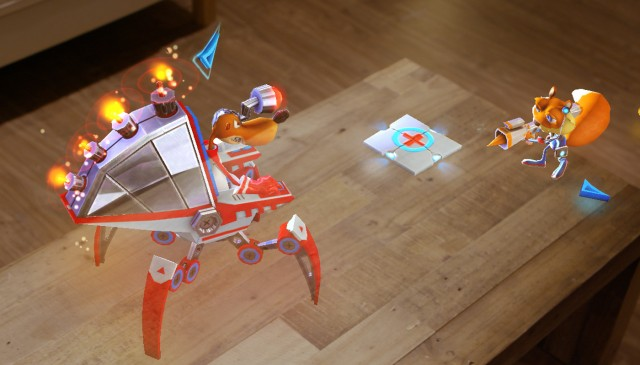
\includegraphics[scale=0.4]{images/youngconker}
\caption{Asobo Studio - Young Conker}
\label{fig:youngconker}
\end{figure}

\paragraph{Réalité augmentée vue au travers}
% Trouver qui l'a inventé et quand
La réalité augmentée vue au travers\cite{milgram1995augmented}, plus communément appelée \emph{See Through Augmented Reality (STAR)}, est une technique de visualisation de la réalité augmentée où les éléments numériques sont vus au travers d'un écran (fig~\ref{sub:STARGO}) ou d'un \emph{HMD} (fig~\ref{sub:STARHolo}). C'est le type de visualisation le plus utilisé actuellement. Toutefois, l'un des défauts majeur de ce type de visualiation est que, la plupart du temps, chaque utilisateur a besoin de son propre écran ou casque pour pouvoir en profiter pleinement ce qui limite grandement les expériences collaboratives. De plus, les principaux inconvénients liés à l'utilisation des écrans s'appliquent également notamment la fatigue visuelle.  

\begin{figure}[H]
    \centering
	\subfloat[Pokémon GO - Vue au travers téléphone]{
      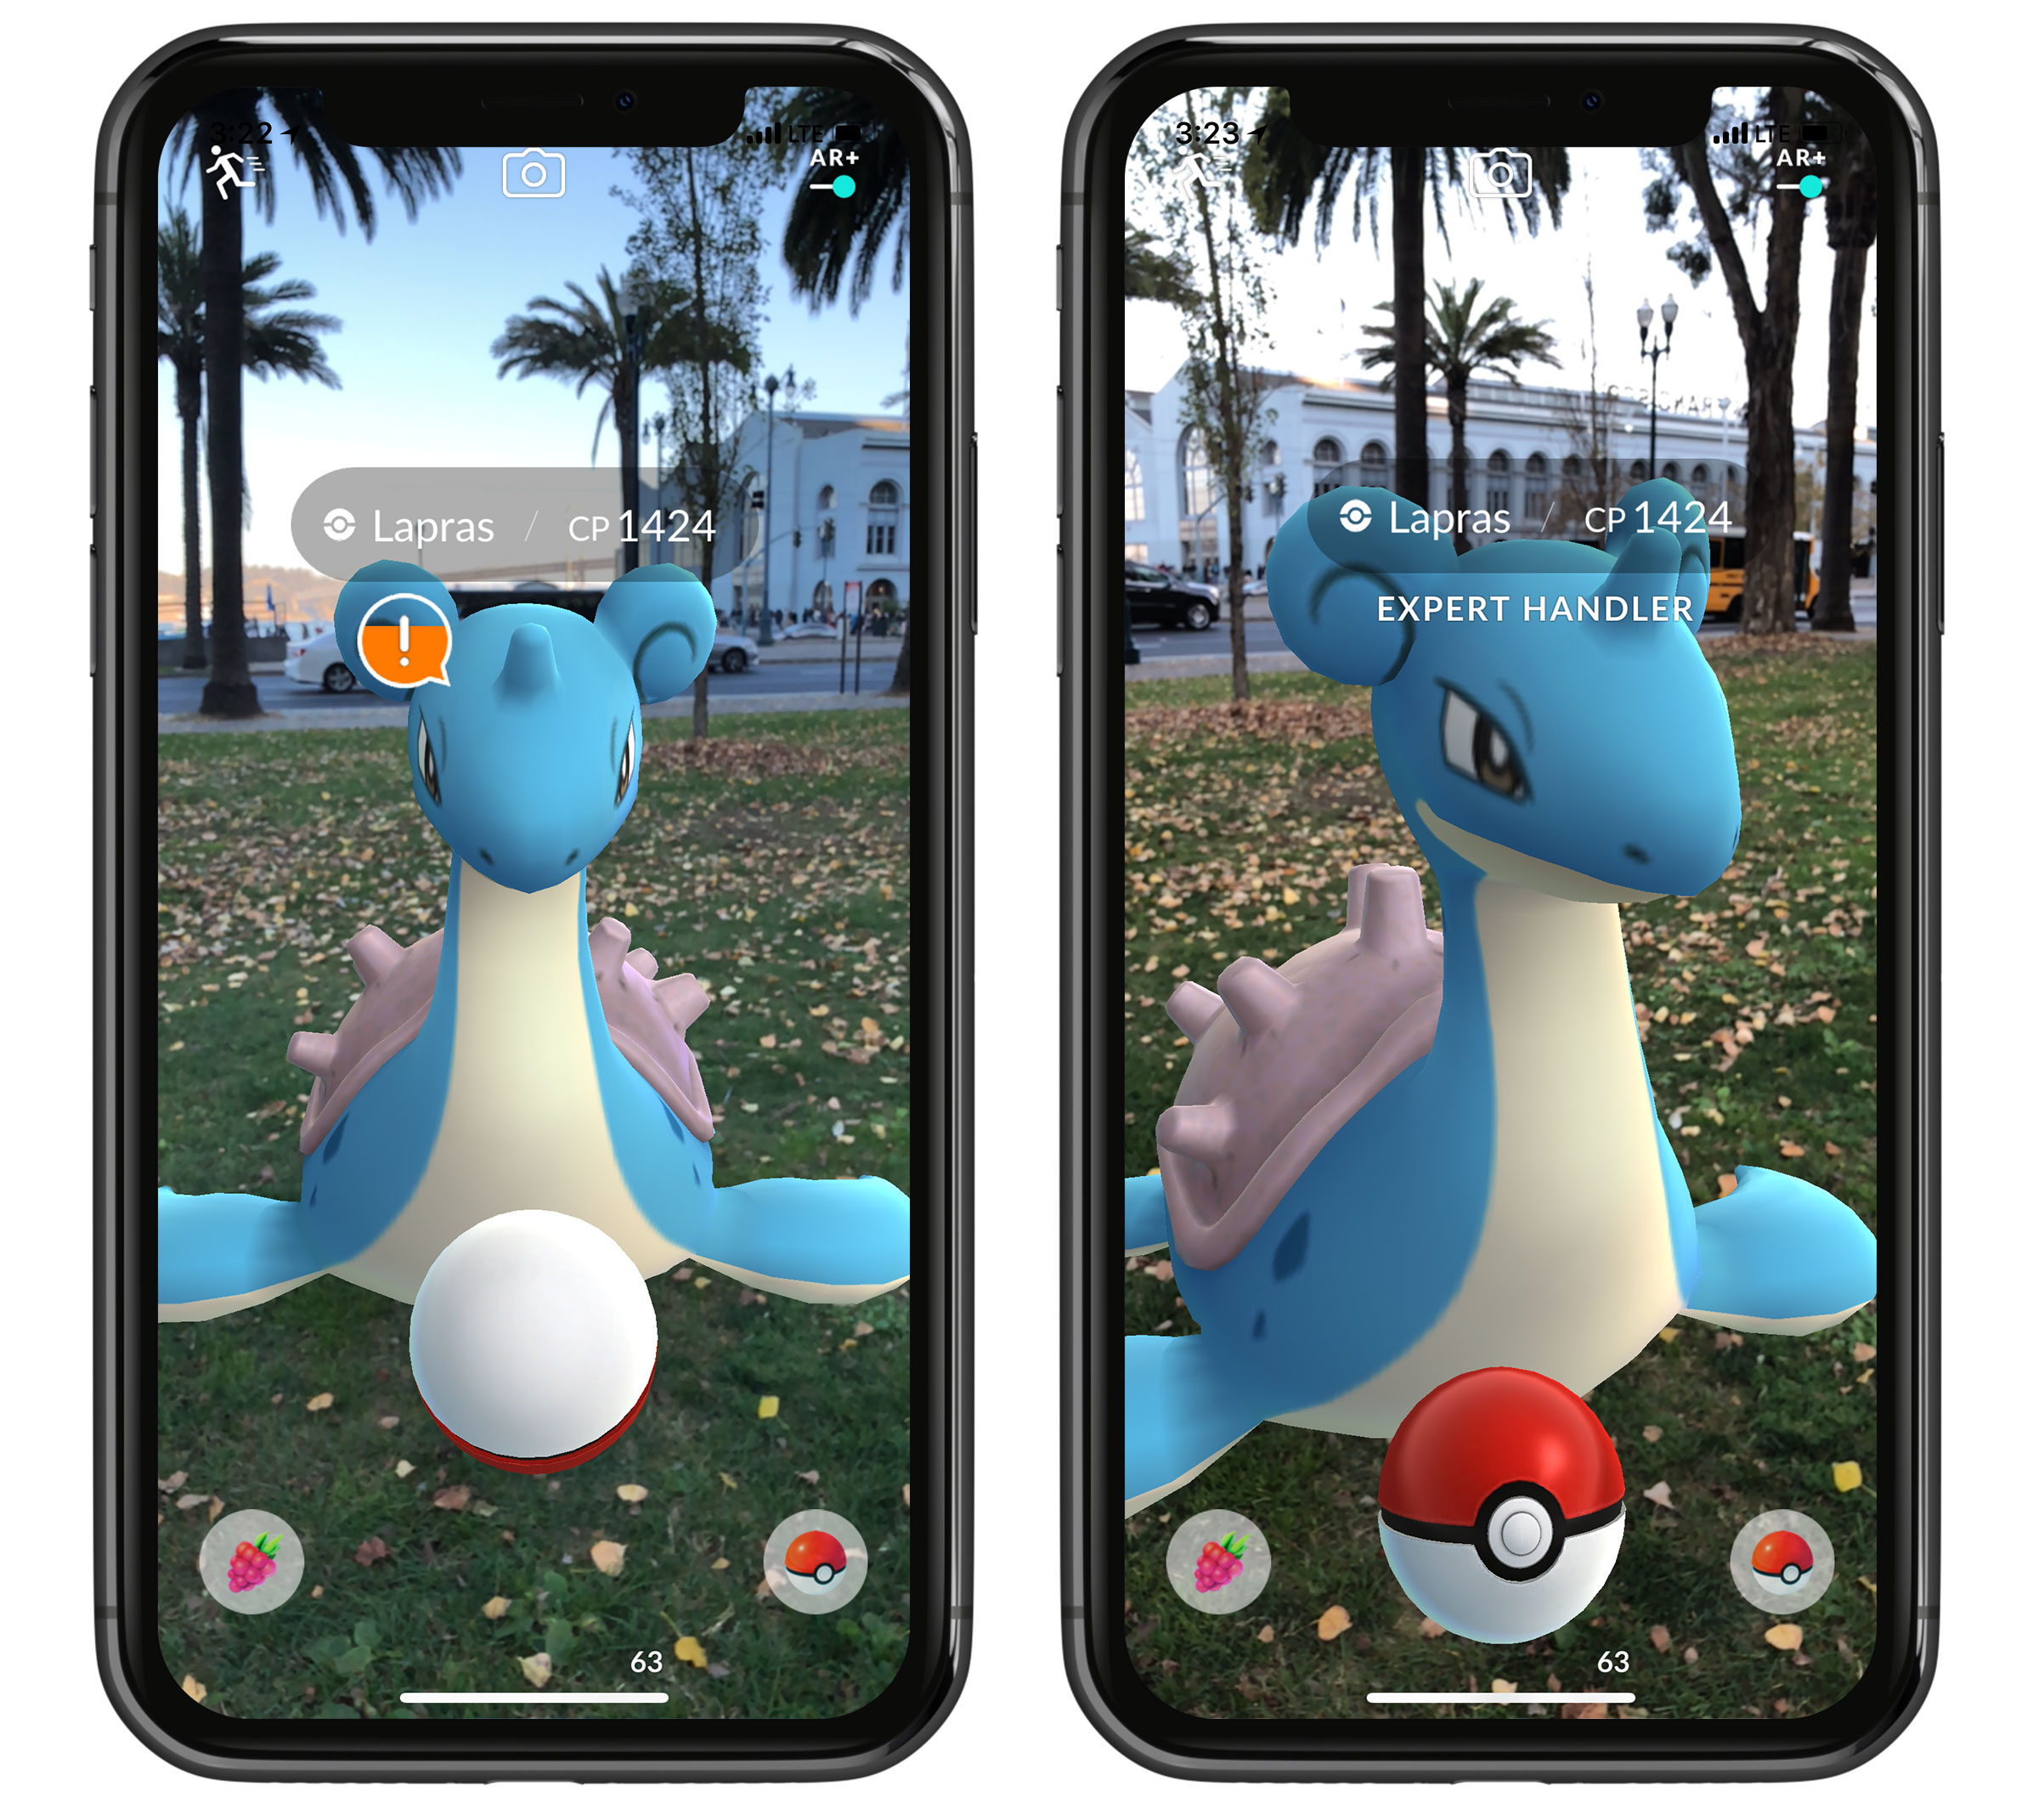
\includegraphics[width=0.45\textwidth]{images/pokemongo}
      \label{sub:STARGO}
      }
    \subfloat[Microsoft HoloLens - Vue au travers casque]{
      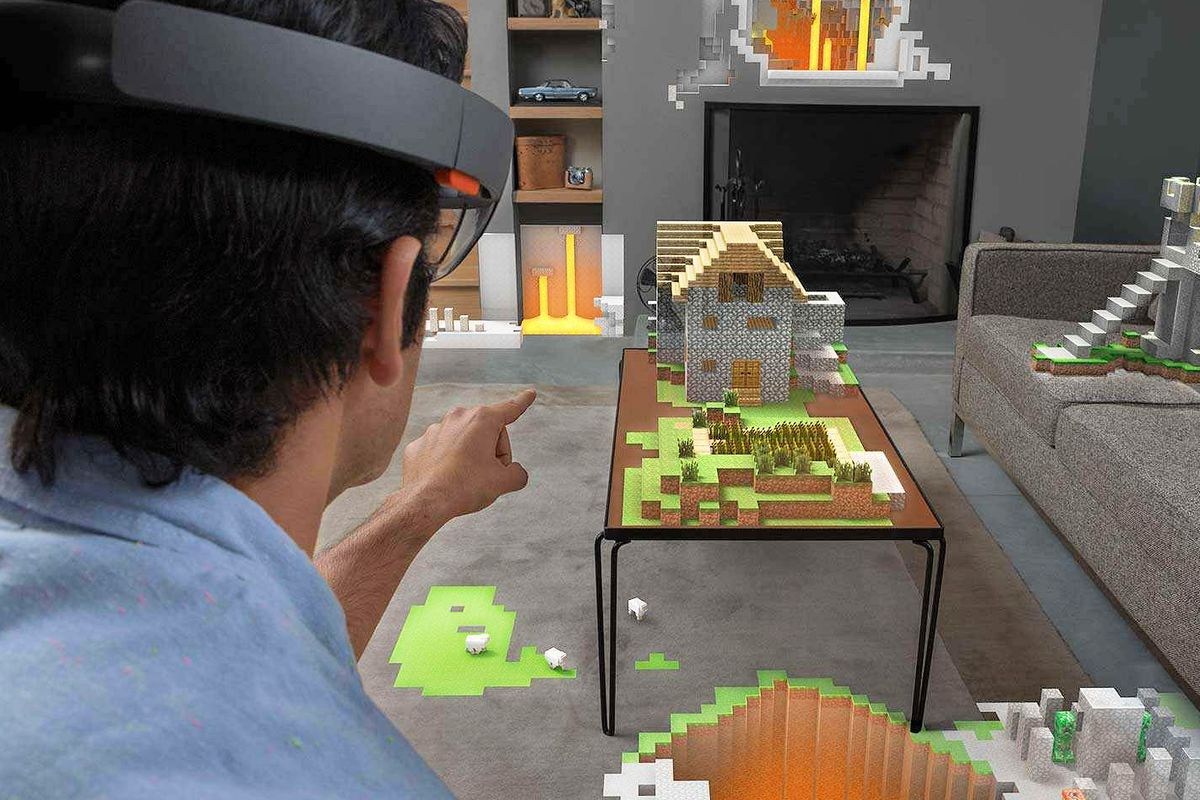
\includegraphics[width=0.45\textwidth]{images/hololens}
      \label{sub:STARHolo}
      }
\caption{Réalité augmentée vue au travers\protect\footnotemark}
\label{fig:STAR}
\end{figure}
\footnotetext{Source: \href{https://pokemongolive.com/fr/}{Pokemon GO} et \href{https://www.microsoft.com/fr-fr/hololens}{Microsoft HoloLens}}

\paragraph{Réalité augmentée spatiale}
% Trouver qui l'a inventé et quand
La réalité augmentée spatiale\cite{bimber2005spatial}, plus communément appelée \emph{Spatial Augmented Reality (SAR)} est une technique de visualisation de la réalité augmentée se basant sur un dispositif de projection. Les éléments virtuels qui viennent "augmenter" le monde réel sont alors projetés dans l'espace (fig~\ref{fig:SAR}), d'où le terme "spatiale". Cette notion d'augmentation de l'espace tend à rendre cette technologie naturellement collaborative car les projections ne dépendent pas d'un dispositif visuel personnel et sont donc obligatoirement partagées. La SAR permet aussi de favoriser le développement d'interfaces tangibles. En effet, la visualisation se faisant directement sur des objets physiques, la tendance à développer des interfaces en communion avec ceux-ci est très forte car très naturelle.

\begin{figure}[H]
\centering
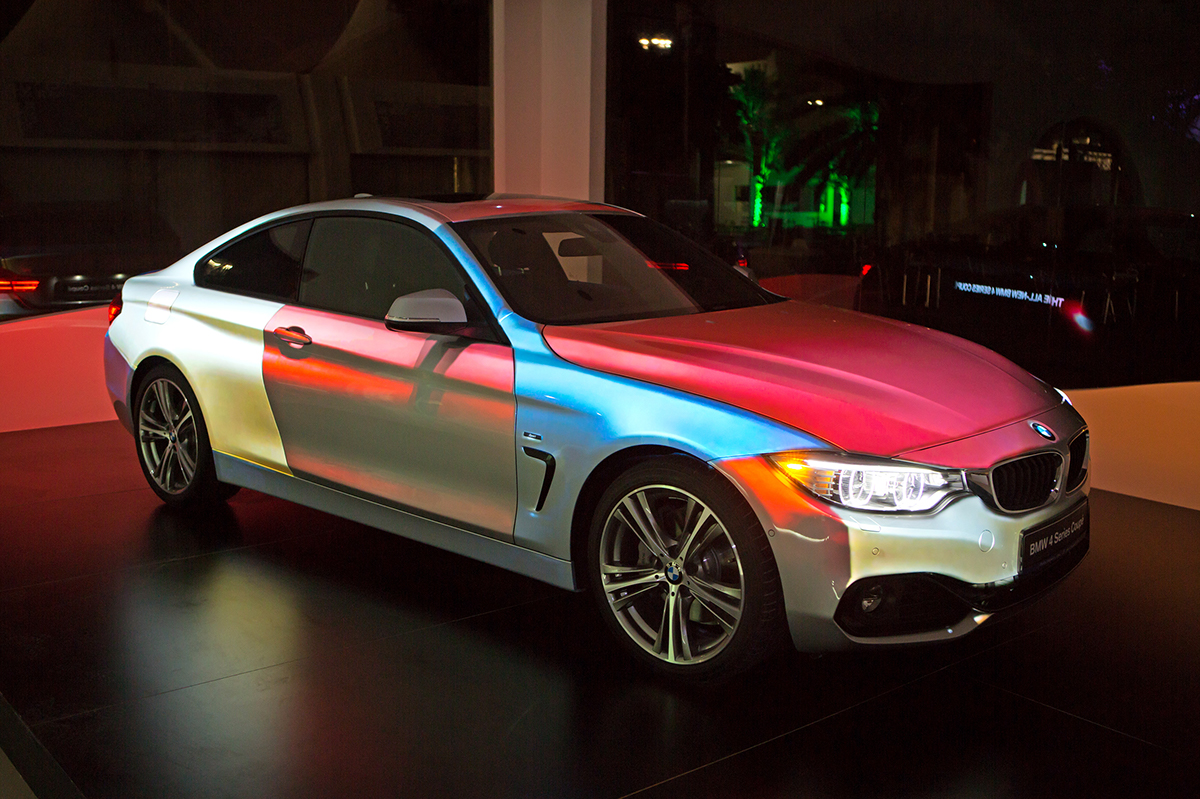
\includegraphics[width=0.5\textwidth]{images/SARMappingCar2}
\caption{Présentation d'une voiture en utilisant de la réalité augmentée spatiale\protect\footnotemark}
\label{fig:SAR}
\end{figure}
\footnotetext{Source: {Google Image}}

\paragraph{Interface tangible}
Une interface utilisateur tangible\cite{ishii2008tangible} ou \emph{Tangible User Interface (TUI)} est une interface utilisateur via laquelle des objets physiques, ou encore le toucher, permettent de manipuler des données numériques (fig~\ref{sub:TUI}). Les interfaces utilisateurs tangibles remplacent très souvent les interfaces utilisateurs graphiques (fig~\ref{sub:GUI}) ou \emph{Graphical User Interface (GUI)} dans la plupart des applications de réalité augmentée car elles fournissent un contrôle direct à l'utilisateur sur ce qu'il souhaite manipuler (par opposition au contrôle indirect tel que la souris, nécessaire à la manipulation des GUI).

\begin{figure}[H]
    \centering
	\subfloat[Interface Utilisateur Graphique (GUI)]{
      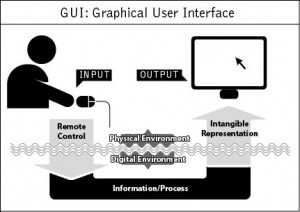
\includegraphics[width=0.45\textwidth]{images/GUI}
      \label{sub:GUI}
      }
    \subfloat[Interface Utilisateur Tangible (TUI)]{
      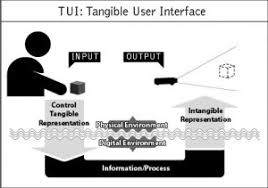
\includegraphics[width=0.45\textwidth]{images/TUI}
      \label{sub:TUI}
      }
\caption{Différences des interfaces utilisateurs\protect\footnotemark}
\label{fig:GUITUI}
\end{figure}
\footnotetext{Source: \href{http://iconlibrary.iconshock.com/design/from-gui-to-tui/}{Icon Library - From GUI to TUI}}

\paragraph{Calcul haute performance}
Le calcul haute performance ou \emph{General-Purpose computing on Graphics Processing Units (GPGPU)} désigne une méthode de calcul utilisant la carte graphique (GPU) plutôt que le processeur (CPU Figure~\ref{fig:gpgpu}. Cette technique permet de bénéficier de la puissance de la carte graphique afin de réaliser du calcul en parallèle et est très souvent utilisée pour la plupart des traitements lourds tels que le rendu d'une scène 3D, l'encodage de vidéo, les simulations physiques (particules) etc. Cette technique repose sur le grand nombre de cœurs présents dans les cartes graphiques (contrairement aux processeurs) et sur la capacité de chacun de ces cœurs à effectuer des opérations simples de manière très efficace. Le calcul haute performance ne peut cependant pas se passer du CPU qui va principalement être utilisé pour récolter et transférer les données traitées ou à traiter.

\begin{figure}[H]
\centering
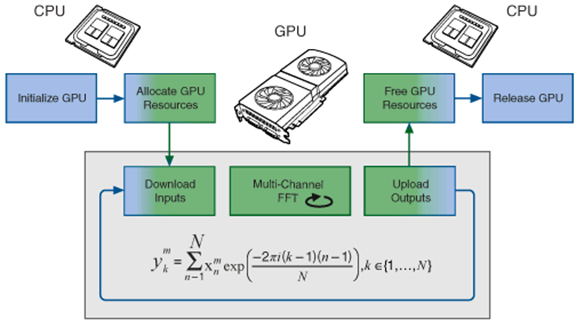
\includegraphics[scale=0.7]{images/gpuworkflow}
\caption{Exemple de calcul de la FFT sur GPU\protect\footnotemark}
\label{fig:gpgpu}
\end{figure}
\footnotetext{Source: \href{http://www.ni.com/white-paper/14077/fr/}{National Instruments}}
